\section{Preliminaries}

Henceforth let {\em billiard 3-periodics} refer to the 1d family of Poncelet triangles interscribed between pair of confocal ellipses $\E$ and $\E_c$ given by:
\[ \E:\frac{x^2}{a^2}+\frac{y^2}{b^2}-1=0,\;\;\;\E_c:\frac{x^2}{a_c^2}+\frac{y^2}{b_c^2}-1=0\]
where $c^2=a^2-b^2=a_c^2-b_c^2$.

Billiard N-periodics classically conserve  perimeter $L$ and Joachimsthal's constant $J$. The latter one is equivalent to stating all trajectory segments are tangent to a confocal caustic, see \cite[Thm 4.4]{sergei91} and \cite{arnold2020-joachim}.
When $N=3$, we can derive these explicitly using the vertex parametrization given in \cref{eq:02-p2}.
 
\begin{proposition}
For billiard 3-periodics, the perimeter and Joachimsthal's constant are given by:

\begin{equation*}
J=\frac{\sqrt{2\delta-a^2-b^2}}{c^2},\;\;\;L=2(\delta+a^2+b^2)J
\label{eqn:n3-L-J}
\end{equation*}
where $\delta=\sqrt{a^4-a^2b^2+b^4}$.
\end{proposition}

\begin{proof} We compute the values considering  an isosceles 3-periodic with $P_1=[a,0]$, and

% {\small  
% \begin{equation}\label{eq:isosceles_3orbit}
%  \;  P_2   =\left[-\frac {{a}^{2}\sqrt {2\,\delta-{a}^{2}-{b}^{2}}}{c^2},   
%	\frac { \left(\delta  -{a}^{2}\right) b}{c^2}\right],\;\;
%	    P_3= \left[{-\frac {{a}^{2}\sqrt {2\,\delta-{a}^{2}-{b}^{2} }}{c^2}},
%	{\frac { \left(  {a}^{2}-\delta \right) %b}{c^2}}\right]
%\end{equation}
 %}%
 {\small 
 \begin{equation} \label{eq:orbita3-isosceles}
 P_2=\left[   {\frac {a \left(  {b}^{2}-\delta \right) }{   a^2-b^2 
 			  }},{\frac {{b}^{2}\sqrt {2 \delta -{a}^{2}-{b}^{2}\,
 				}}{{a}^{2}-{b}^{2}}} 
 	\right], \;\; P_3=\left[  {\frac {a \left(  {b}^{2}-\delta \right) }{   a^2-b^2   
 	}},-{\frac {{b}^{2}\sqrt {2\delta-{a}^{2}-{b}^{2} 
 				}}{{a}^{2}-{b}^{2}}} 
 	\right]
 	\end{equation}
 	}
 	We have that
 	\[L=|P_2-P_3|+2|P_1-P_2|,\;\;
 	 J=\langle \frac{P_1-P_3}{|P_1-P_3|},[\frac{1}{a},0]\rangle\]
 	 Straightforward calculations using the vertex parametrization in \cref{eq:02-p2}, leads to the stated result.
%\textcolor{red}{ronaldo: CAS+parametrization}
\end{proof}

Henceforth the oft-ocurring quantity $\delta$ will be referred to as the Darboux constant. An interesting geometric interpretation for it appears in \cref{prop:02-delta}.

%\noindent Note: the use of $J$ in this chapter refers to its value for the $N=3$ case.

\section{Caustic semi-axes}

The Cayley condition for a concentric, axis parallel (CAP) pair of ellipses to admit a 3-periodic family is given by:

\begin{equation} \frac{a_c}{a}+\frac{b_c}{b}=1
\label{eqn:n3-cayley}
\end{equation}

In turn, this constrains the semi-axes of the confocal caustic.

\begin{proposition}
The semi-axes $a_c,b_c$ of the confocal caustic are given by:
\begin{align*}
a_c=&\frac{a\left(\delta-{b}^{2}\right)}{c^2},\;\;\;\;
b_c=\frac{b\left({a}^{2}-\delta\right)}{c^2}\cdot
\end{align*}
\label{prop:02-n3-caustic}
\end{proposition}

When $a=b$, we have that $a_c=b_c=a/2$.

\begin{proposition}
The semi-axes $a$ and $b$ of the ellipse in terms of the semi-axes $a_c$ and $b_c$ of the confocal ellipse are given by:
\begin{align*}
a&= -\frac{1}{2} \sqrt{w_1} + \frac{1}{2} \sqrt{ w_2 -\frac{ 2 a_c^3 - 4 c^2a_c}{\sqrt{w_1}} } +\frac{a_c}{2},\;\; b=\sqrt{a^2-c^2}\\
w_1&=a_c^2-(4 c a_c b_c)^{\frac{2}{3}},\;\; w_2=2 a_c^2+ (4 c a_c b_c)^{\frac{2}{3}}
\end{align*}
The implicit equation that defines $a$ above is the quartic  given by
\[c^2( a_c^2   - 2   a_c   a )+ a^2(2a_c a  - a^2)=0\]
\label{prop:02-caustic-to-billiard}
\end{proposition}

\section{Incenter and excenter loci}
\label{sec:02-inc-exc-loci}

\begin{figure}
    \centering
    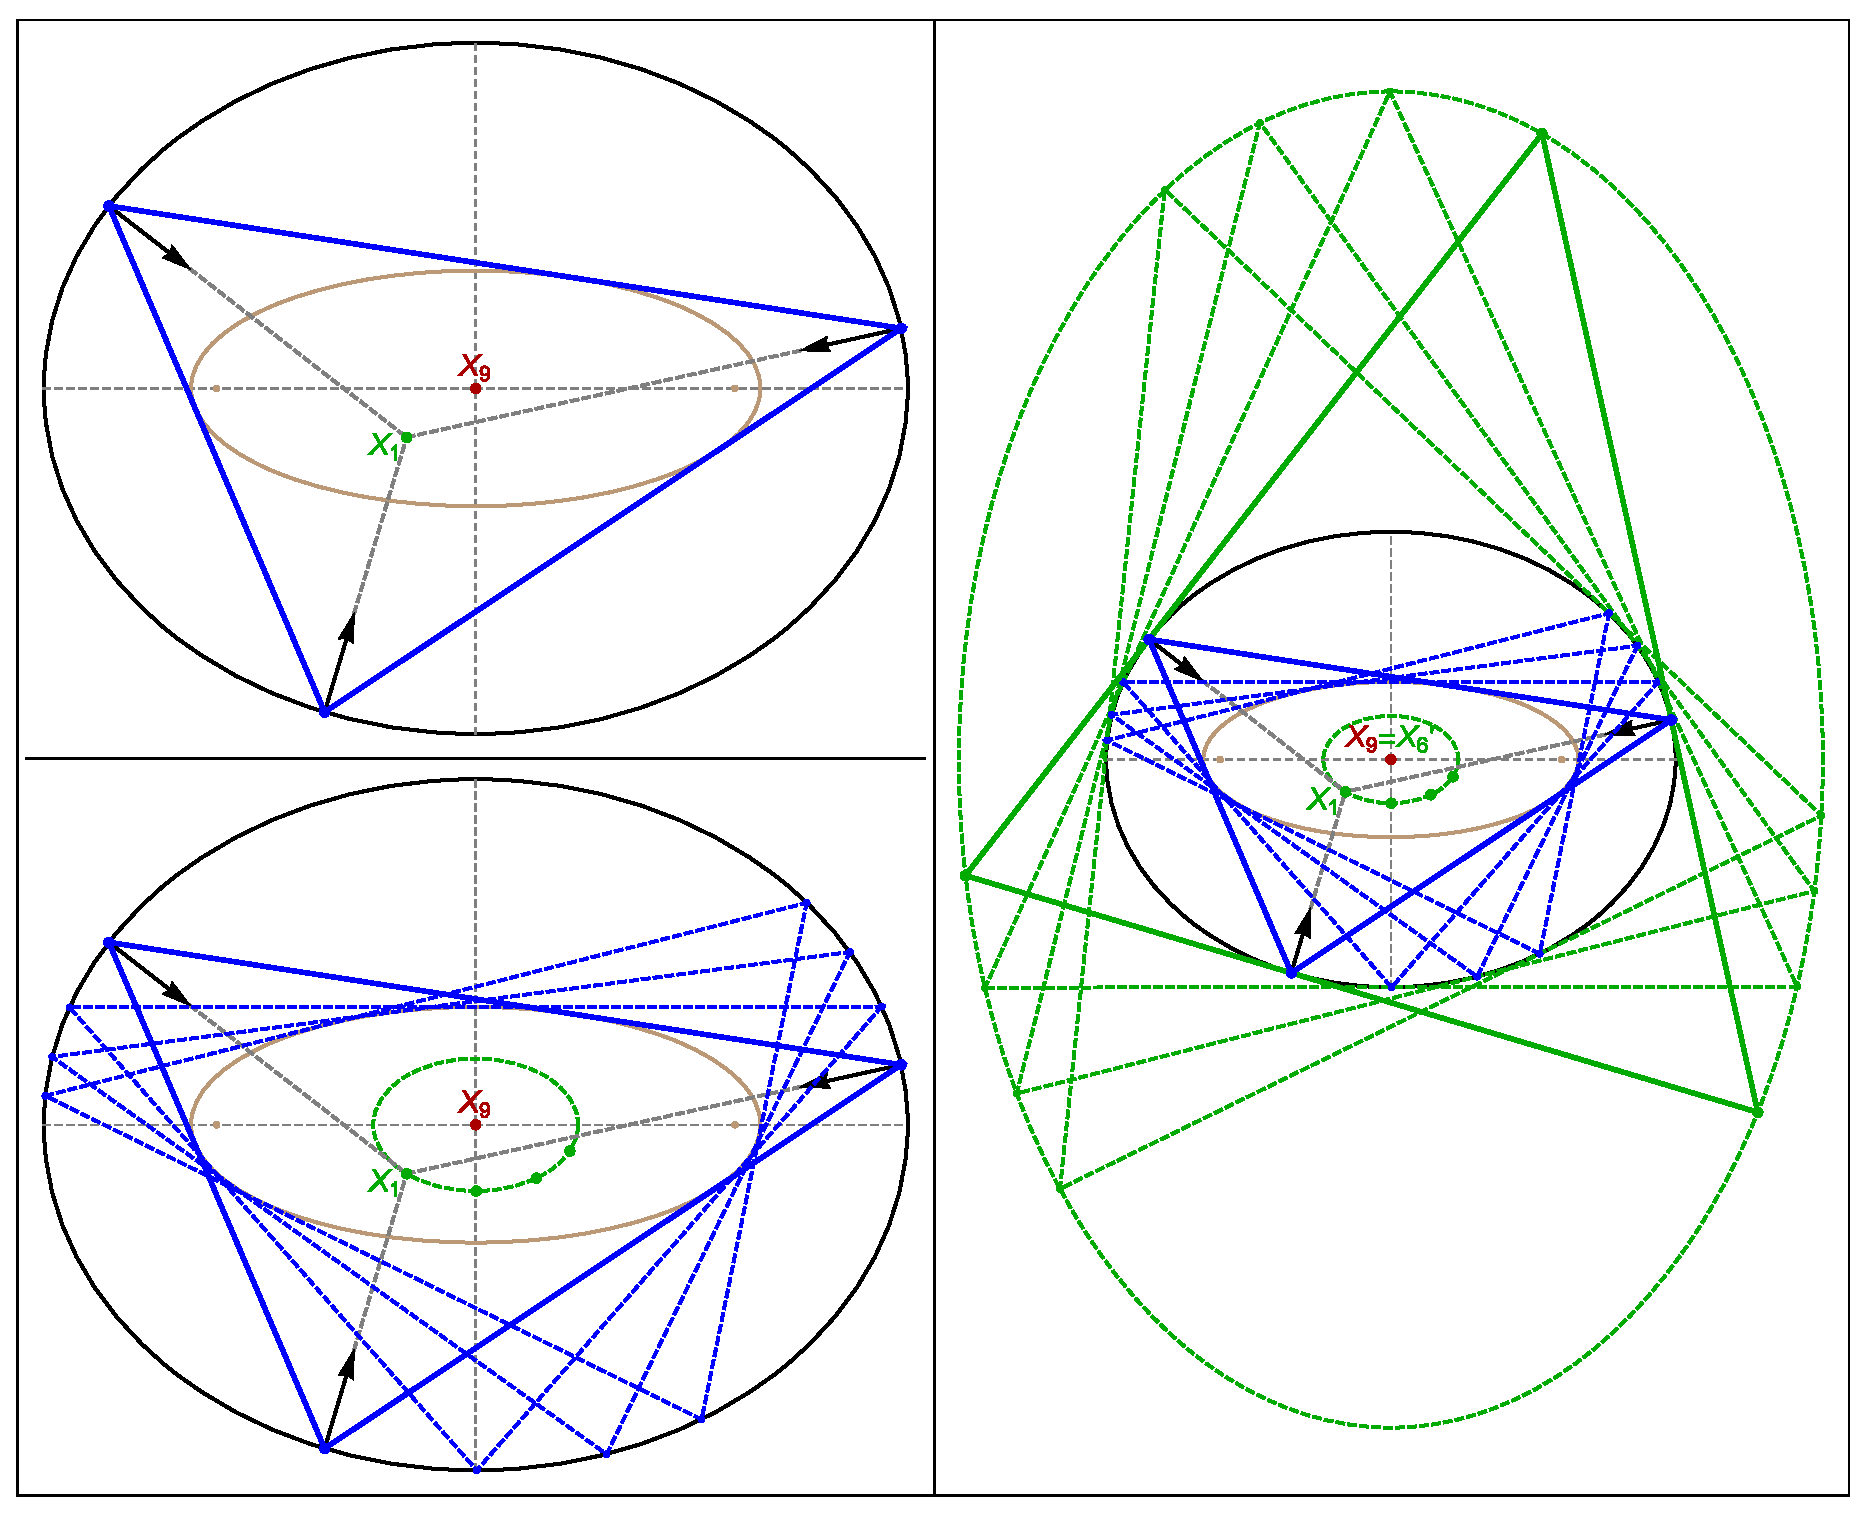
\includegraphics[width=\textwidth]{pics_02_010_billiard_grid}
    \caption{\textbf{Top Left:} An elliptic billiard 3-periodic (solid blue) is shown inscribed in an outer ellipse (black) and a confocal caustic (brown). Graves' theorem implies its internal angles will be bisected by ellipse normals (black arrows). Also shown is the incenter $X_1$ defined as the intersection of said bisectors. \textbf{Bottom Left:} Poncelet's porism implies a 1d family of such triangles exists. Some samples are shown (dashed blue). A classic invariant is  perimeter. The Mittenpunkt $X_9$ remains stationary at the center. The incenter $X_1$ sweeps an ellipse (dashed green). \textbf{Right:} The excentral triangle (solid green) has sides perpendicular to the bisectors. Over billiard 3-periodics, the excentral is of variable perimeter. Its vertices (known as the ``excenters'') also sweep an ellipse (dashed green) whose aspect ratio is the reciprocal of that of the incenter locus. The Symmedian point $X_6'$ of the excentral triangle coincides with $X_9$ of the reference and is therefore stationary. \href{https://bit.ly/3gWl3CI}{Live}}
    \label{fig:billiard-grid}
\end{figure}

An intriguing phenomenon is that over billiard 3-periodics, the locus of both incenter and the excenters are ellipses, as was initially detected experimentally (see an early \href{https://youtu.be/BBsyM7RnswA}{Video}). This was proved by \cite{olga14} and \cite{garcia2019-incenter}. Indeed, we haven't yet found another Poncelet pair where this is the case, see \cref{conj:07-incenter-excenter-loci}.

Referring to \cref{fig:billiard-grid}:

\begin{theorem}
Over billiard 3-periodics, the locus of the incenter $X_1$ and excenter are ellipses $\E_1$ and $\E_e$ concentric and axis-parallel with the confocal pair whose axes $(a_1,b_1)$ and $(a_e,b_e)$ are given by:
\begin{align*}
a_1 =& \frac{\delta-b^2 }{a},\;\;\;b_1=\frac{a^2-\delta}{b}\\ 
a_e= &\frac{{b}^{2}+\delta}{a},\;\;\;b_e=\frac{{a}^{2}+\delta}{b}
\end{align*}
Furthermore, $\E_1$ and $\E_e$ have reciprocal aspect ratios, i.e., $a_1/b_1=b_e/a_e$.
\label{thm:02-incenter-excenter}
\end{theorem}

\begin{proof}
It follows from the vertex parametrization in \cref{eq:02-p2} and the definition of incenter and excenters. We have that
\[X_1=\frac{s_1 P_1+s_2P_2+s_3P_3}{s_1+s_2+s_3}=
\frac{1}{L}(s_1P_1+s_2P_2+s_3P_3)\]
where $s_1=|P_2-P_3|$, $s_2=|P_1-P_3|$ and $s_3=|P_1-P_2|$.
A careful symbolic analysis shows that $\mathcal{E}_1(X_1)=0$. A similar analysis considering the excenters shows that the locus of the three points is the ellipse $\mathcal{E}_e$ stated.
\end{proof}

\noindent A more general treatment to the above is given in \cref{chap:07-n3-loci}.

\begin{corollary}
The pair $\{\mathcal{E},\mathcal{E}_e\}$ is Ponceletian.
\label{cor:02-excentral-billiard-poncelet}
\end{corollary}

\begin{proof}
Direct from Cayley condition
\[\frac{a}{a_e}+\frac{b}{b_e}=\frac{a^2}{b^2+\delta}+\frac{b^2}{a^2+\delta}= 1\]

\end{proof}

\section{A stationary point}
\label{sec:02-stationary}

The Mittenpunkt $X_9$ is a triangle center where lines from each excenter thru the side midpoint meet. Referring to \cref{fig:02-x9}:
\begin{theorem}
Over the family of 3-periodics in the elliptic billiard, $X_9$ is stationary at the common center.
\end{theorem}

An elegant syntethic proof was kindly contributed by \cite{olga19_mitten}:

\begin{proof}
Let $\E$ be the outer ellipse in the confocal pair, $O$. By definition, the Mittenpunkt $X_9$ is where lines from the excenters $E_i$ through the side midpoints $M_i$ concur. Notice each side is an ellipse chord between tangents to $\E$ seen from the $E_i$ (this is because in the confocal pair the excentral triangle is tangent to $\E$). Consider the image of lines $E_i M_i$ under an affine transform which sends $\E$ to a circle $\Cm'$, let $O'$ be its center. The transformed lines will pass through the midpoints of chords of $\Cm'$ between tangents seen from $E_i'$ (the affine image of $E_i$). By circular symmetry, such lines must also pass through $O'$, and therefore remain stationary. But $O'$ is the affine image of $O$, so the result follows.
\end{proof}

\begin{figure}
     \centering
    \includegraphics[width=\linewidth]{pics_02_020_mitten_proof.pdf}
     \caption{\textbf{Left}: 3-periodic billiard triangle (blue), its excentral triangle (green). The Mittenpunkt $X_9$ is the point of concurrence of lines drawn from the excenters through sides' midpoints $M_i$. \textbf{Right}: the affine image which sends the billiard to a circle. Lines from imaged excenters through sides' midpoints must pass through the origin. Since the latter is stationary, so must be its pre-image $X_9$, which is stationary at the billiard center.  % done
     \href{https://youtu.be/tMrBqfRBYik}{Video}}
     \label{fig:02-x9} 
\end{figure}

\section{Conserved Quantities}

Given a triangle, let $r$ and $R$ denote the radius of its incircle and circumcircle, known as the {\em inradius} and {\em circumradius}, respectively. Over billiard 3-periodics, note these two radii are variable. Referring to \cref{fig:radii}:

\begin{theorem}
$r/R$ is invariant over billiard 3-periodics and given by:
\begin{equation*}
\label{eqn:rovR}
\frac{r}{R}=\frac{2 (\delta-b^2)(a^2-\delta)}{c^4}.
\end{equation*}
\label{thm:02-confocal-rovR}
\end{theorem}

\begin{proof}
The following relation, found in \cite{johnson1960}, holds for any triangle:

\begin{equation*}
 r R=\frac{s_1s_2s_3}{2 L}, 
\end{equation*}

\noindent where $L=s_1+s_2+s_3$ is the perimeter, constant over billiard 3-periodics. Therefore:

\begin{equation}
\frac{r}{R}=\frac{1}{2L} \frac{s_1s_2s_3}{R^2}\cdot
\label{eqn:rovR-cas}
\end{equation}

Next, let $P_1=(a,0)$ be a vertex of an isosceles 3-periodic. Obtain a candidate expression for $r/R$. This yields \eqref{eqn:rovR} exactly. Using the vertex parametrization in \cref{eq:02-p2}, derive an expression for the square of the right-hand side of \eqref{eqn:rovR-cas} as a function of $x_1$ and subtract from it the square of \eqref{eqn:rovR}. In  \cite{garcia2020-new-properties}
it is shown $\left(s_1s_2s_3/R^2\right)^2$ is rational on $x_1$. For simplification, use $R=s_1 s_2 s_3/(4A)$, where $A$ is the triangle area. With a CAS, show said difference is identically zero for all $x_1\in(-a,a)$.
\end{proof}


\begin{figure}
    \centering
    \includegraphics[width=\textwidth]{pics_02_030_radii}
    \caption{The incircle (green), circumcircle (purple), and 9-point (Euler's) circle (pink) of a billiard triangle (blue). These are centered on $X_1$, $X_3$, and $X_5$, respectively. Their radii are the inradius $r$, circumradius $R$, and 9-point circle radius $r_9=2R$. Over the family, the ratio $r/R$ is invariant. In turn this implies an invariant sum of cosines. \href{https://bit.ly/337hvpf}{Live}}
    \label{fig:radii}
\end{figure}

Let $\theta_i$, $r$, $R$, and $A$ denote the ith internal angle, inradius, circumradius, and area of a reference triangle. Primed quantities refer to the excentral triangle. The relations below, appearing in  \cite{johnson1960},  hold for any triangle:

\begin{align}
\sum_{i=1}^{3}{\cos\theta_i}&=1+\frac{r}{R} \label{eqn:02-sum-cos} \\
\prod_{i=1}^{3}{\cos\theta_i'}&=\frac{r}{4R} \label{eqn:02-exc-prod-cos} \\
\frac{A}{A'}&=\frac{r}{2R} \label{eqn:02-area-ratio}
\end{align}

\begin{corollary}
Over billiard 3-periodics, also invariant are the sum of 3-periodic cosines, the product of excentral cosines, and the ratio of excentral-to-3-periodic areas.
\label{cor:02-rOvR}
\end{corollary}

Direct calculations yields an expression for the invariant sum of cosines in terms of elliptic billiard constants $J$ and $L$.

\begin{corollary}
$\sum_{i=1}^{3}{\cos\theta_i}=J L - 3$
\end{corollary}

At it will be seen later in \cref{chap:05-billiard}, the above generalizes to $J L -N$ for all $N$.

Let $P_i$ be a billiard 3-periodic vertex and $d_{j,i}=|P_i-f_j|$ its distance to billiard focus $f_j$. 

\begin{proposition}
 Over billiard 3-periodics, the following sum is invariant:
\[  \sum\frac{1}{d_{1,i}}=\sum\frac{1}{d_{2,i}}=\frac {{a}^{2}+{b}^{2}+\delta}{a{b}^{
2}}
\]
\label{prop:02-confocal-inv-spokes}
\end{proposition}

\begin{proof}
Direct computation with CAS using vertex parametrization given in \cref{sec:02-vertex-para}.
\end{proof}

Let $P=(x,y)$ be a point on an ellipse with semi-axes $a,b$. In \cite[Ellipse]{mw}, the curvature at $P$ is expressed both in terms of its coordinates and the distances $d_1,d_2$ to the foci as follows:

\begin{equation}
\kappa = \frac{1}{a^2 b^2} \left(\frac{x^2}{a^4}+\frac{y^2}{b^4}\right)^{-3/2} = \frac{a b}{(d_1 d_2)^{3/2}}
\label{eqn:02=curv}
\end{equation}

Let $\kappa_i$ denote the billiard ellipse curvature at vertex $P_i$ of a Poncelet 3-periodic. From the above and \cref{prop:02-confocal-inv-spokes} obtain:

\begin{corollary}
Over billiard 3-periodics, the following quantity is conserved:
\[ \sum_{i=1}^3{\kappa_i^\frac{2}{3}} =\frac{ a^2 + b^2 + \delta}{ (ab)^{\frac{4}{3}} }\]
\label{prop:02-confocal-curv-sum}
\end{corollary}

\section{An interpretation for \torp{$\delta$}{delta}}

The Darboux constant $\delta$ appearing above has a curious geometric interpretation. Recall the power of a point $Q$ with respect to a circle $\Cm=(C_0,R_0)$ is given by $|Q-C_0|^2-R_0^2$, see \cite[Circle Power]{mw}. Let $\Cm$ denote the (moving) circumcircle of billiard 3-periodic, and $O=X_9$ the billiard center.

\begin{proposition}
The power of $O$ with respect to $\Cm$ is constant and equal to $-\delta$.
\label{prop:02-delta}
\end{proposition}

\begin{proof}
Consider an isosceles billiard 3-periodic given by \cref{eq:orbita3-isosceles}.
	Its circumcircle will be centered at $C_0=[ {\frac { {b}^{2}-\delta}{2b}},0]$ with circumradius $R_0=\frac {{b}^{2}+\delta}{2b}.$
	Therefore, the power of the center of the ellipse with respect to the circumcircle is given by  
	$$|OC_0|^2-R_0^2=\left(\frac { {b}^{2}-\delta}{2b}\right)^2 - \left(\frac {{b}^{2}+\delta}{2b}\right)^2=-\delta.$$
	
	The stated invariance is confirmed with a CAS using the vertex parametrization in \cref{eq:02-p2}.  
%	\textcolor{red}{localizar depois}
\end{proof}



